\documentclass[12pt, a4paper, oneside]{ctexart}
\usepackage{amsmath, amsthm, amssymb, graphicx}
\usepackage[bookmarks=true, colorlinks, citecolor=blue, linkcolor=black]{hyperref}
\usepackage[margin = 25mm]{geometry}
\usepackage{setspace}
\usepackage{listings}
\usepackage{cite}
% 导言区
\title{粒子在双delta势垒下的共振隧穿及其应用}
\date{\today}
\author{成员:孙陶庵,张钧赫,彭智贤,翟梦瑶,李凤,马璐,樊欣怡}
\begin{document}
\begin{spacing}{2.0}
\maketitle
\section{摘要}
本文基于使用薛定谔方程解决一维粒子的能量本征态这一知识点
研究粒子在穿透双delta势垒时出现的共振状态,
并且通过计算对反射系数和透射系数对其进行验证和可视化
并且讨论了该共振态在不同前沿科技上的应用。
\section{引言}
在经典力学中,当入射粒子能量小于势垒能量时,粒子将无法穿透势垒,全都会被反射回去。
但在量子力学中,即使粒子能量小于势垒能量,粒子也有一定的概率能够穿过势垒,
当粒子入射能量合适时,会出现共振隧穿的情况。\par
我们通过写出势垒外部的能量本征方程求解出三个区域带有四个未知量的波函数表达式,
再通过两个delta势垒处波函数及波函数导数的关系列出四个含有未知量的方程进而确定出波函数。\par
同时可以求出各个反射和透射系数代入波函数进行可视化操作。
除此之外,也通过可视化呈现了不同能量取值下各个区域的波函数情况。
\section{计算推导}
设质量为$m$,能量为$E(E> 0)$的粒子从左入射,碰到$\delta$势垒:\\
\begin{center}
  $V=\alpha[\delta(x+a)+\delta(x-a)]$
\end{center}
\begin{figure}[htbp]
    \centering
    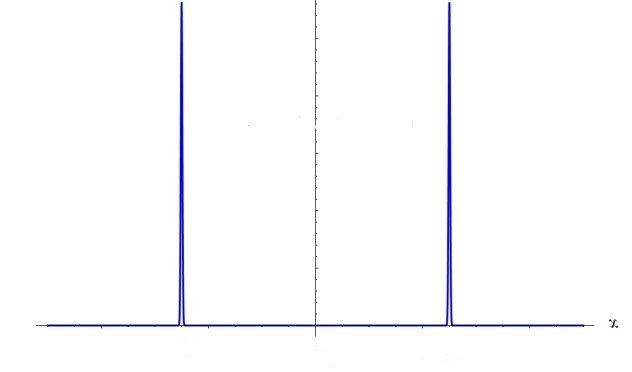
\includegraphics[width=8cm]{delta.jpg}
    \caption{$V=\alpha[\delta(x+a)+\delta(x-a)]$}
\end{figure}
\subsection{求解}

我们可以利用散射矩阵\cite{griffiths_schroeter_2018}\cite{RN05}来得到关系:
$\begin{bmatrix}
    F\\
    G
  \end{bmatrix}
  \begin{bmatrix}
   M_{11} &M_{12} \\
   M_{21} &M_{22}
  \end{bmatrix}
  =\begin{bmatrix}
    A\\
    B
  \end{bmatrix}$\\
这样有反射系数$R=\left | \frac{M_{12}}{M_{22}} \right |^2 $
以及透射系数$T=\left|\frac{1}{M_{22}}\right|^2$。\\
\begin{figure}[htbp]
    \centering
    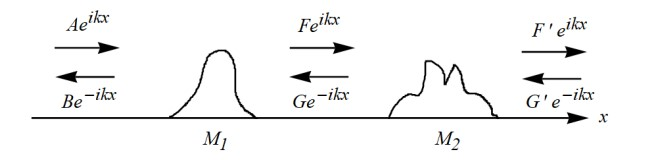
\includegraphics[width=8cm]{double potential.jpg}
    \caption{双势垒}
\end{figure}

而对于一多重势垒(假设是双势,见图2)有:
$\begin{bmatrix}
    F\\
    G
  \end{bmatrix}
  M_1
  =\begin{bmatrix}
    A\\
    B
  \end{bmatrix},
  \begin{bmatrix}
    F'\\
    G'
  \end{bmatrix}
  M_2
  =\begin{bmatrix}
    F\\
    G
  \end{bmatrix}
$
则可以看出:\\
\begin{center}
  $
\begin{bmatrix}
    F'\\
    G'
  \end{bmatrix}
  M_2 M_1
  =\begin{bmatrix}
    A\\
    B
  \end{bmatrix}
$\\
\end{center}

所以$M=M_2 M_1$\\
因此,我们可以首先考虑单个delta势垒$V=\alpha\delta(x-a)$
\\对于薛定谔方程:
\begin{center}
  $i\hbar\frac{\partial \Psi}{\partial t} = -\frac{\hbar^2}{2 m} \frac{\partial^2 \Psi}{\partial x^2}+V(x) \Psi(x,t)$
\end{center}
分离变量
\begin{center}
$\Psi(x,t)=\psi(x)\phi(t)$
\end{center}
\begin{center}
$i\hbar\psi\frac{d\phi}{dt}=-\frac{\hbar^2}{2m} \phi\frac{d^2 \psi}{dx^2}+V\psi\phi$\\
$\Rightarrow i\hbar\frac{\dot\phi}{\phi}=-\frac{\hbar^2}{2m}\frac{\ddot\psi}{\psi}+V=E $\\
$\left\{\begin{matrix}    i\hbar\frac{\dot\phi}{\phi}=E \\     -\frac{\hbar^2}{2m}\frac{\ddot\psi}{\psi}+V=E  \end{matrix}\right. $\\
\end{center}
将势能V带入,得
\begin{center}
$\left\{\begin{matrix}    i\hbar\frac{\dot\phi}{\phi}=E \\     -\frac{\hbar^2}{2m}\frac{\ddot\psi}{\psi}+\alpha\delta(x-a)=E  \end{matrix}\right. $\\
\end{center}
E为满足边界条件的特征值,
\begin{center}
$ \frac{\partial^2\psi}{\partial x^2}+\frac{2m}{\hbar^2} \left\{E-\alpha\delta(x-a)\right\}\psi=0$   (1)\\
\end{center}
如果$x\neq a$,
$\Rightarrow \frac{\partial^2\psi}{\partial x^2}+\frac{2mE}{\hbar^2}\psi=0 $
会有以下解
\begin{center}
$\psi(x)= \left\{\begin{matrix}    Ae^{ikx}+Be^{-ikx},x<-a \\  Fe^{ikx}+Ge^{-ikx},x>a\\  \end{matrix}\right. ,k=\frac{\sqrt{2mE}}{\hbar}$\\
\end{center}
并且此时有边界条件:
\begin{center}
$ \lim\limits_{x \to a^-}\psi(x)=\lim\limits_{x\to a^+}\psi(x)$
\end{center}
这样可得:
\begin{center}
$ Ae^{ika}+Be^{-ika}=Fe^{ika}+Ge^{-ika} $  (1)
\end{center}
而其他的条件可对(1)式积分,范围从$-a-\epsilon$到$-a+\epsilon$
\begin{center}
$\displaystyle\int^{-a+\epsilon}_{-a-\epsilon}\left\{\frac{\partial^2\psi}{\partial x^2}\right\}=-\frac{2m}{\hbar^2}[E-\alpha\delta(x-a)]\psi(x) dx $\\
$\displaystyle\int^{-a+\epsilon}_{-a-\epsilon}\frac{\partial^2\psi}{\partial x^2}dx=-\frac{2m}{\hbar^2}\left\{E \displaystyle\int^{-a+\epsilon}_{-a-\epsilon}\psi(x) dx-\alpha\displaystyle\int^{-a+\epsilon}_{-a-\epsilon}[\delta(x-a)]\psi(x) dx\right\}$\\
$\frac{\mathrm{d}\psi}{\mathrm{d}x}\bigg|^{a+\epsilon}_{a-\epsilon}=-\frac{2m}{\hbar^2}\bigg[E\psi(a)\displaystyle\int^{a+\epsilon}_{a-\epsilon}\mathrm{d}x-\alpha\psi(a)\bigg]$\\
$\frac{\mathrm{d}\psi}{\mathrm{d}x}\bigg|^{a+\epsilon}_{a-\epsilon}=-\frac{2m}{\hbar^2}[E\psi(a)(2\epsilon)-\alpha\psi(a)]$ , 令$\epsilon \to 0$\\
$\frac{\mathrm{d}\psi}{\mathrm{dx}}\bigg|^{-a^+}_{-a^-}=\frac{2m\alpha}{\hbar^2}\psi(a)=0$\\
$\frac{2m\alpha}{\hbar^2}\psi(a)=\lim\limits_{x \to a^+}\frac{\mathrm{d}\psi}{\mathrm{d}x}-\lim\limits_{x \to a^-}\frac{\mathrm{d}\psi}{\mathrm{d}x}$\\
$ik(Fe^{ika}-Ge^{-ika})-ik(Ae^{ika}-Be^{-ika})=\frac{2m\alpha}{\hbar^2}(Ae^{ika}+Be^{-ika})$   (2)\\
\end{center}
由(1)(2)式求出F和G的表达式,
最终可以得到
\begin{center}
$\left\{\begin{matrix} F=\frac{k\hbar^2-im\alpha}{k\hbar^2}A-\frac{im\alpha}{k\hbar^2}e^{-2ika}B
     \\ G=\frac{im\alpha}{k\hbar^2}e^{2ika}A+\frac{k\hbar^2+im\alpha}{k\hbar^2}B \end{matrix}\right.  $\\
    \end{center}
可以看出
$\begin{bmatrix}
    F\\
    G
  \end{bmatrix}
  \begin{bmatrix}
    \frac{k\hbar^2-im\alpha}{k\hbar^2} &-\frac{im\alpha}{k\hbar^2}e^{-2ika} \\
    \frac{im\alpha}{k\hbar^2}e^{2ika} &\frac{k\hbar^2+im\alpha}{k\hbar^2}
  \end{bmatrix}
  =\begin{bmatrix}
    A\\
    B
  \end{bmatrix}$\\
即\\
$M_1=
\begin{bmatrix}
    \frac{k\hbar^2-im\alpha}{k\hbar^2} &-\frac{im\alpha}{k\hbar^2}e^{-2ika} \\
    \frac{im\alpha}{k\hbar^2}e^{2ika} &\frac{k\hbar^2+im\alpha}{k\hbar^2}
  \end{bmatrix}
$
\\而对于$V=\alpha\delta(x+a)$也是同样的算法,这里不赘述,其矩阵:
$M_2=
\begin{bmatrix}
    \frac{k\hbar^2-im\alpha}{k\hbar^2} &-\frac{im\alpha}{k\hbar^2}e^{2ika} \\
    \frac{im\alpha}{k\hbar^2}e^{-2ika} &\frac{k\hbar^2+im\alpha}{k\hbar^2}
\end{bmatrix}
$
所以\\
$
M=M_2 M_1=
\begin{bmatrix}
    \frac{(k\hbar^2-im\alpha)^2+m^2\alpha^2e^{4ika}}{k^2\hbar^4}&\frac{-im\alpha(k\hbar^2-im\alpha)e^{-2ika}-im\alpha(k\hbar^2+im\alpha)e^{2ika}}{k^2\hbar^4}\\
    \frac{im\alpha(k\hbar^2-im\alpha)e^{-2ika}+im\alpha(k\hbar^2+im\alpha)e^{2ika}}{k^2\hbar^4}&\frac{(k\hbar^2+im\alpha)^2+m^2\alpha^2e^{-4ika}}{k^2\hbar^4}
\end{bmatrix}
$
则
$T=\left|\frac{1}{M_{22}}\right|^2=\\
\frac{4 \hbar^4 m^2 E^2}{4 \hbar^4 m^2 E^2 + 4 \hbar^2 m^3 E \alpha^2 + 2 m^4 \alpha^4 + 
4 \hbar^2 m^3 E \alpha^2 \cos[\frac{4\sqrt{2} a \sqrt{mx}}{\hbar}] - 
2 m^4 \alpha^4 \cos[\frac{4\sqrt{2} a \sqrt{m x}}{\hbar}] - 
4 \sqrt{2} \hbar m^3 \sqrt{m x} \alpha^3 \sin[\frac{4\sqrt{2} a \sqrt{m1 x}}{\hbar}]}$\\
$R=\left|\frac{M_{12}}{M_{22}}\right|^2=\\
\frac{m\alpha^2(-2\hbar^2 x - 
m \alpha^2 + (-2 \hbar^2 x + m \alpha^2) \cos[\frac{4\sqrt{2}a\sqrt{mx}}{\hbar}] + 
2 \sqrt{2} \hbar \sqrt{mx}\alpha \sin[\frac{4\sqrt{2}a\sqrt{mx}}{\hbar}])}{-2 \hbar^4 x^2 - 2 \hbar^2 m x \alpha^2 - m^2 \alpha^4 + 
m \alpha^2[ (-2 \hbar^2 x + m \alpha^2) \cos[\frac{4\sqrt{2}a\sqrt{mx}}{\hbar}] 
+ 2 \sqrt{2} \hbar \sqrt{mx}\alpha \sin[\frac{4\sqrt{2}a\sqrt{mx}}{\hbar}]]}
$\\
\begin{figure}[htbp]
    \centering
    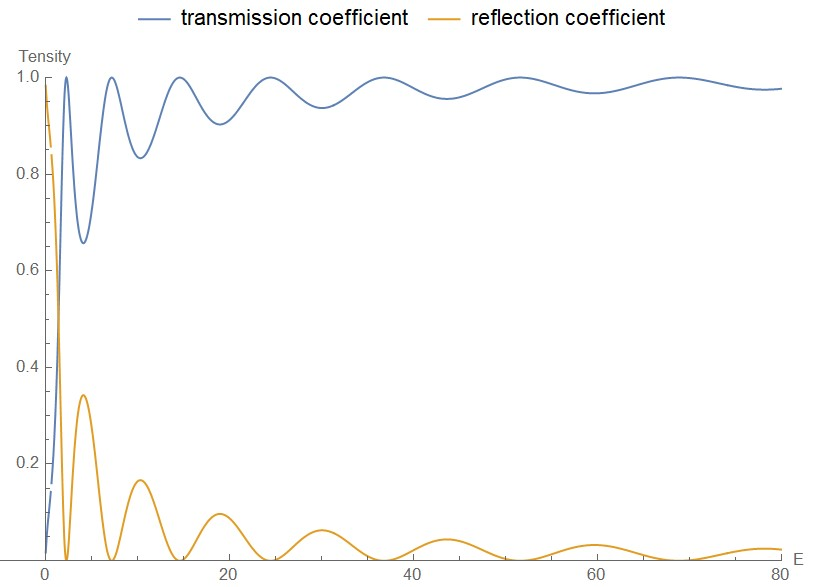
\includegraphics[width=8cm]{transreflect.jpg}
    \caption{反透射关系图}
\end{figure}
图3是在$m=\hbar^2,a=\hbar,\alpha=\frac{1}{\hbar}$的特殊情况。\\
并且说明:
1.粒子能量较低时,反射系数随势垒常数增大而减小。
随着入射粒子能量的增大,反射系数的变化逐渐减缓,
说明势垒高度对粒子反射率的影响逐渐减小。
当入射粒子能量与势垒高相近时,反射系数在无穷远处收敛于0,
相当于变化周期无穷大。
2.粒子能量较低时,透射系数随势垒常数增大而减小。
随着入射粒子能量的增大,透射系数的变化逐渐减缓,
说明势垒高度对粒子透射率的影响逐渐减小。
当入射粒子能量与势垒高相近时,透射系数在无穷远处收敛于1,
相当于变化周期无穷大。\cite{key}
\section{双$\delta$势的应用}
\subsection{$\delta$势对基于反平行不对称磁势垒半导体微结构的电子动量滤波器的影响}
\cite{QIN2021127571}通过探究原子层掺杂技术实现$\delta$势对滤波器件的影响,结果表明,该滤波器对某一电位敏感,
因为器件中的电子所经历的有效电位取决于$\delta$电位。
	
\begin{figure}[htbp]
	\centering
	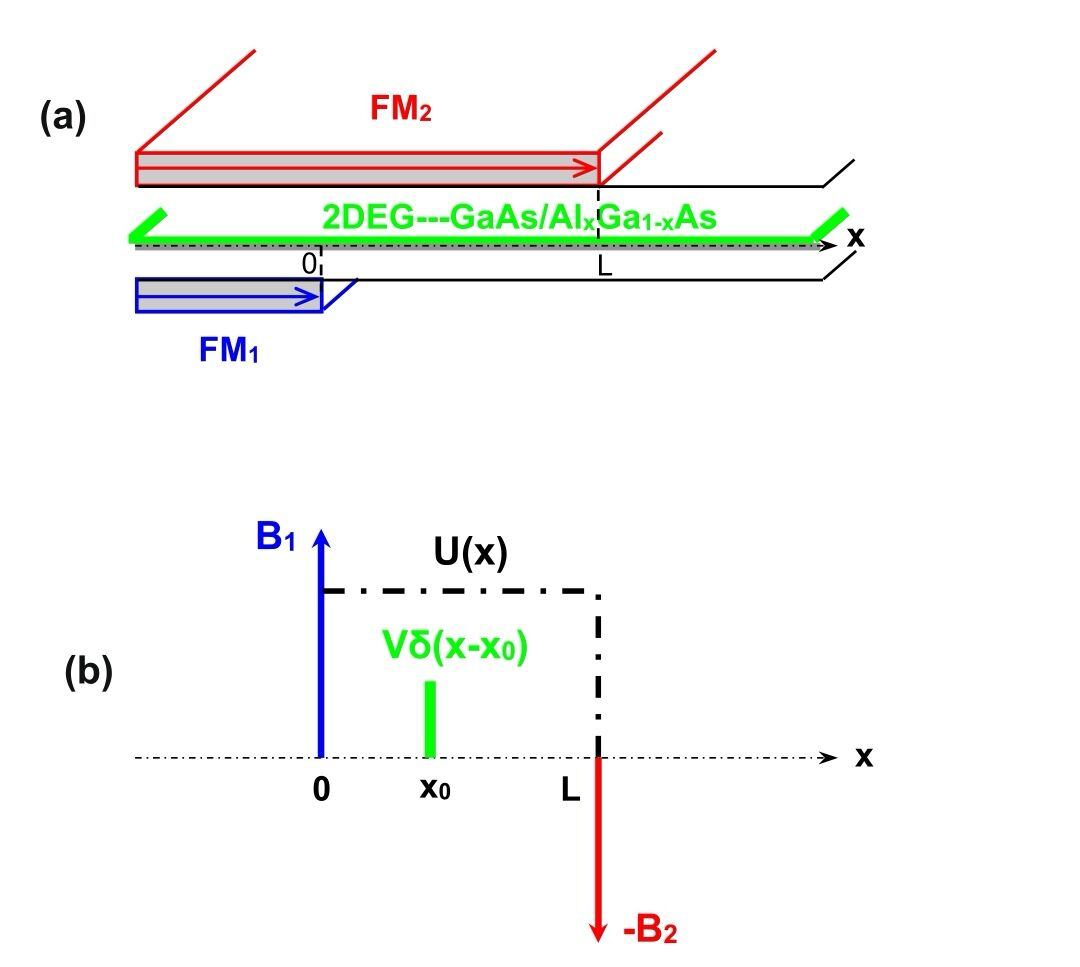
\includegraphics[width=8cm]{alpha123.jpg}
	\caption{MCSM的$\delta$势模型}
\end{figure}
如图1,MCSM可以构建在半导体异质结构的表面。其模型如(b)所示,其中$\delta$嵌入MCSM中。
	
通过在ALDT的帮助下引入$\delta$势,可从理论上研究电子动量滤波器的操纵。还发现,WVF效率可通过改变$\delta$势的位置来控制。因此可以提出一种用于纳米电子器件应用的可调节电子动量滤波器。
	
\subsection{晶格中双$\delta$函数势的透射系数的应用}
\cite{YANETKA1999371}由薛定谔——万尼尔方程,电势定义为两个强度不等的$\delta$函数之和,从该解导出透射系数表达式。  对于相应的单$\delta$函数势,透射系数在其最大值处大于而在最小值处小于透射系数。
半导体双势垒结构的传输已经得到了广泛的研究。在垂直于界面的方向上,双势垒结构最常被一维系统中的矩形双势垒建模。
传输系数的近似解析表达式几乎只能在 WKB 近似内获得,
另一方面,通过对称双$\delta$势垒的传输进行了深入研究,现代计算机能够以相对容易的数值计算实际势能的传输系数。
然而,传输系数的解析表达式仍然具有指导价值。这就是为什么双$\delta$屏障也被用作双屏障结构的原型。
虽然双$\delta$势垒是矩形双势垒的一种非常简化的形式,但它仍然可以让人们深入了解通过双势垒的传输。

\section{总结}
共振态能级是指在垒间区域的值远大于垒外区域的值,而与此相应的能量就称为共振态能级。
对于双$\delta$势垒,存在无穷多个分立能级,而在我们给出的条件下也同时可以看出$T+R=1$的关系。
在这篇文章中给出了M矩阵的的解法,并用其来求解两个大小相等的$\delta$势,
而如果要求解强度不等的势(例如$V=\alpha \delta(x-a)+\beta \delta(x+a)$),只需要将另一个势前面的系数$\alpha$改掉即可,第三个第四个势也是如此
我们在处理势垒的时候,可以利用S矩阵或者M矩阵来简化求解过程(理论上这可以推广到无穷多个势),从而得到我们需要的透射系数及反射系数以及波函数。
而有关S矩阵\cite{enwiki:1074717524}和M矩阵\cite{RN03}的内容会留到参考文献里面。
\newpage
\section{附录}
\subsection{Mathemetica代码}
\begin{lstlisting}
h = (6.63*10^-34)/(2 \[Pi]);
m = h^2;
a = h;
T[x_] := (((Sqrt[2 m x]/
      h)^2 h^4)/((Sqrt[2 m x]/h h^2 + I m \[Alpha])^2 + 
     m^2 \[Alpha]^2 Exp[-4 I Sqrt[2 m x]/h a])) (((Sqrt[2 m x]/
      h)^2 h^4)/((Sqrt[2 m x]/h h^2 - I m \[Alpha])^2 + 
     m^2 \[Alpha]^2 Exp[4 I Sqrt[2 m x]/h a]));
R[x_] := ((-I m \[Alpha] (Sqrt[2 m x]/h h^2 - 
        I m \[Alpha]) Exp[-2 I Sqrt[2 m x]/h a] - 
     I m \[Alpha] (Sqrt[2 m x]/h h^2 + I m \[Alpha]) Exp[
       2 I Sqrt[2 m x]/h a])/((Sqrt[2 m x]/h h^2 + I m \[Alpha])^2 + 
     m^2 \[Alpha]^2 Exp[-4 I Sqrt[2 m x]/h a])) ((
    I m \[Alpha] (Sqrt[2 m x]/h h^2 + I m \[Alpha]) Exp[
       2 I Sqrt[2 m x]/h a] + 
     I m \[Alpha] (Sqrt[2 m x]/h h^2 - I m \[Alpha]) Exp[-2 I Sqrt[
        2 m x]/h a])/((Sqrt[2 m x]/h h^2 - I m \[Alpha])^2 + 
     m^2 \[Alpha]^2 Exp[4 I Sqrt[2 m x]/h a]));
Plot[{T[x/h^2], R[x/h^2]}, {x, -20, 100},
 AxesLabel -> {"E", "Tensity"},
 PlotRange -> {{-5, 80}, {0, 1}},
 PlotLegends -> 
  Placed[{"transmission coefficient", "reflection coefficient"}, 
   Above],
 PlotLegends -> "Expressions"
 ]

\end{lstlisting}
组长打分: \\
1.张钧赫 93\\
2.彭智贤 96\\
3.翟梦瑶 95\\
4.李凤   95\\
5.马璐   95\\
6.樊欣怡 96\\
\end{spacing}

\bibliographystyle{IEEEtran}
\bibliography{re1}

\end{document}